\section{Attribute selection}
\subsection{Impact}
% TODO expliquer ce qu'on calcule. le gain d'info là et qu'on utilise un test a alpha=0.5 pour verifier qui est mieux
\begin{frame}
 \frametitle{Impact of attribute selection}
 \framesubtitle{Linux}
 \begin{center}
  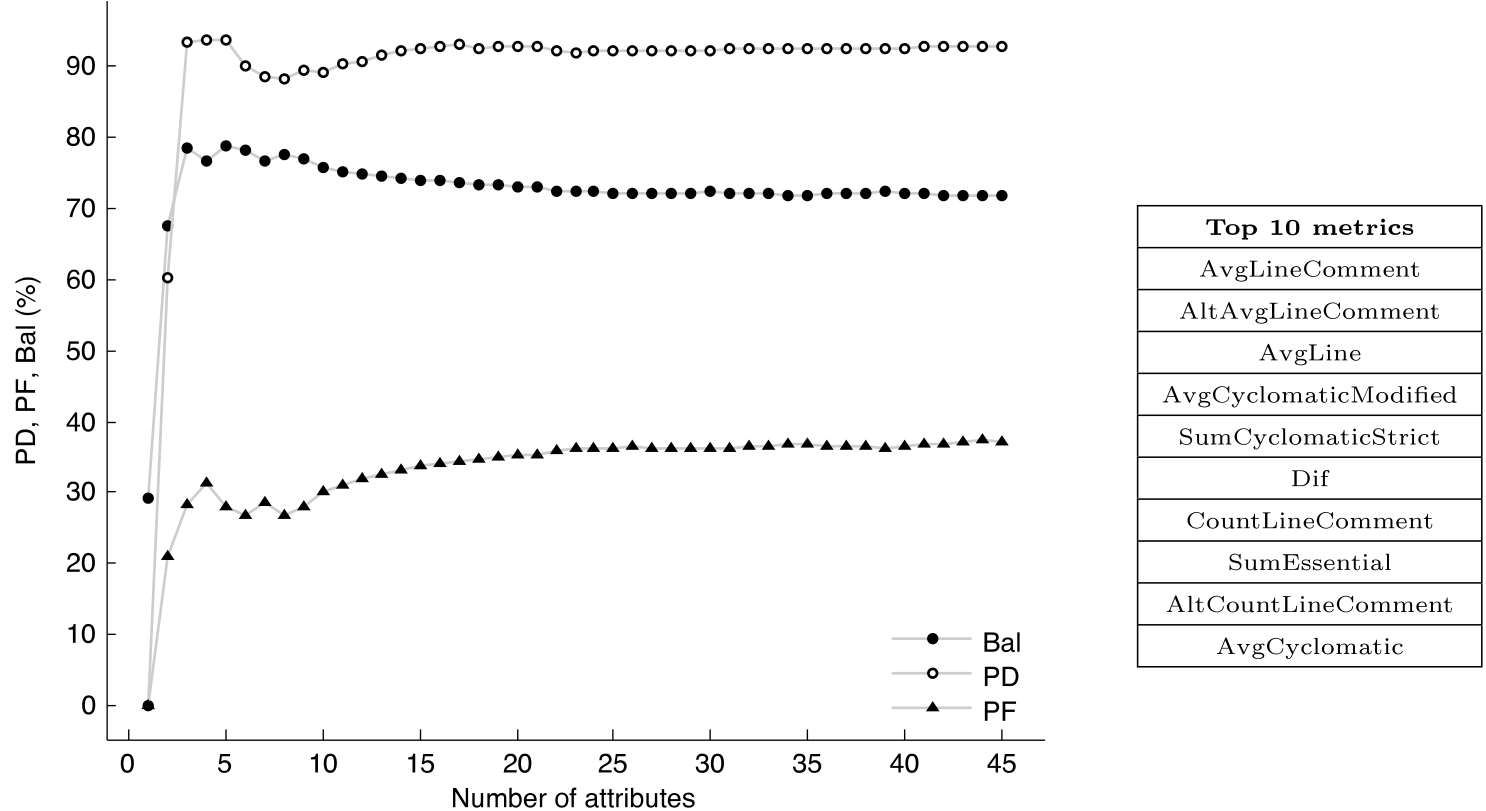
\includegraphics[width=\textwidth]{figures/attributesLinux.png}
 \end{center}
\end{frame}

\begin{frame}
 \frametitle{Impact of attribute selection}
 \framesubtitle{MySQL}
 \begin{center}
  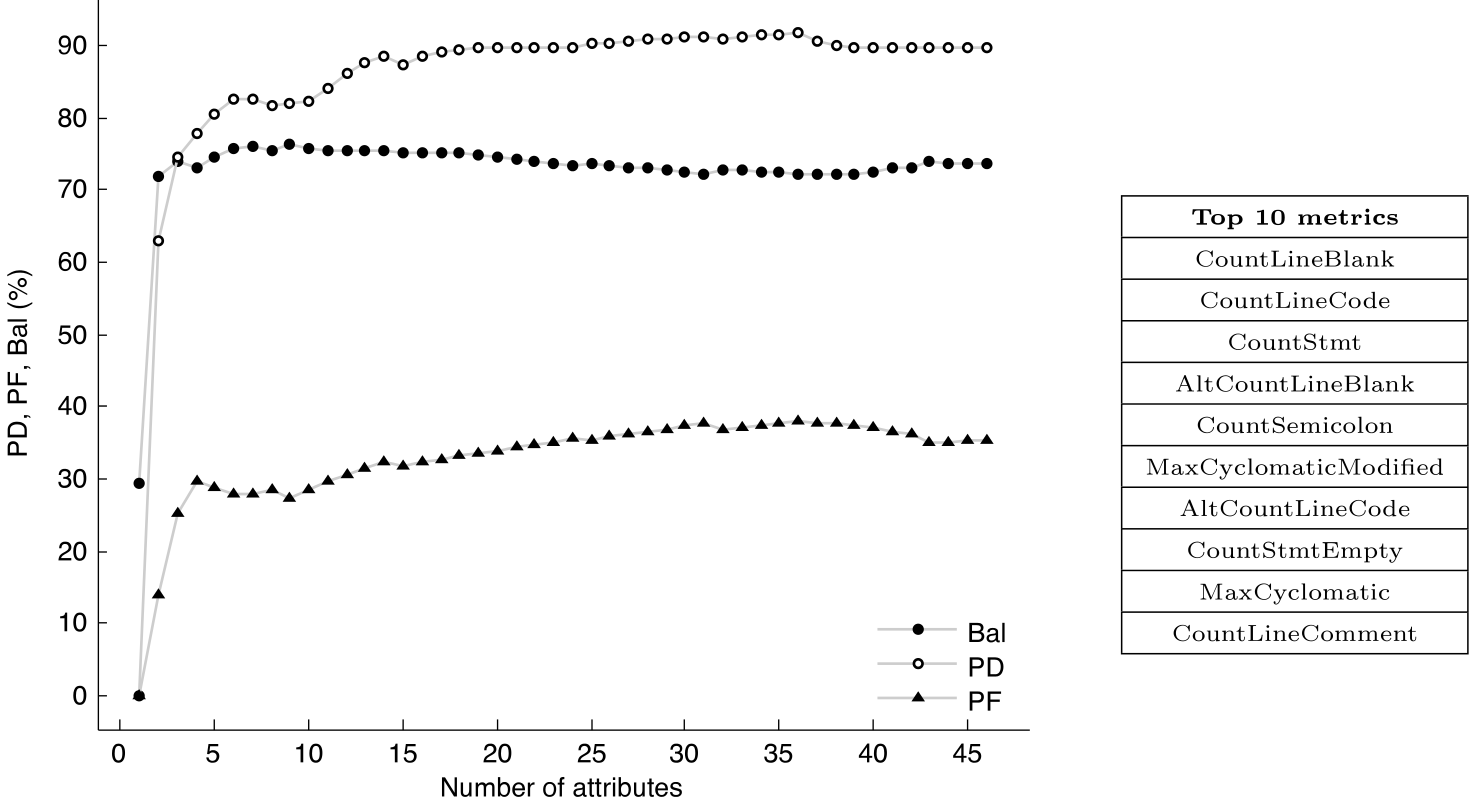
\includegraphics[width=\textwidth]{figures/attributesMysql.png}
 \end{center}
\end{frame}

\begin{frame}
 \frametitle{Impact of attribute selection}
 \framesubtitle{CARDAMOM}
 \begin{center}
  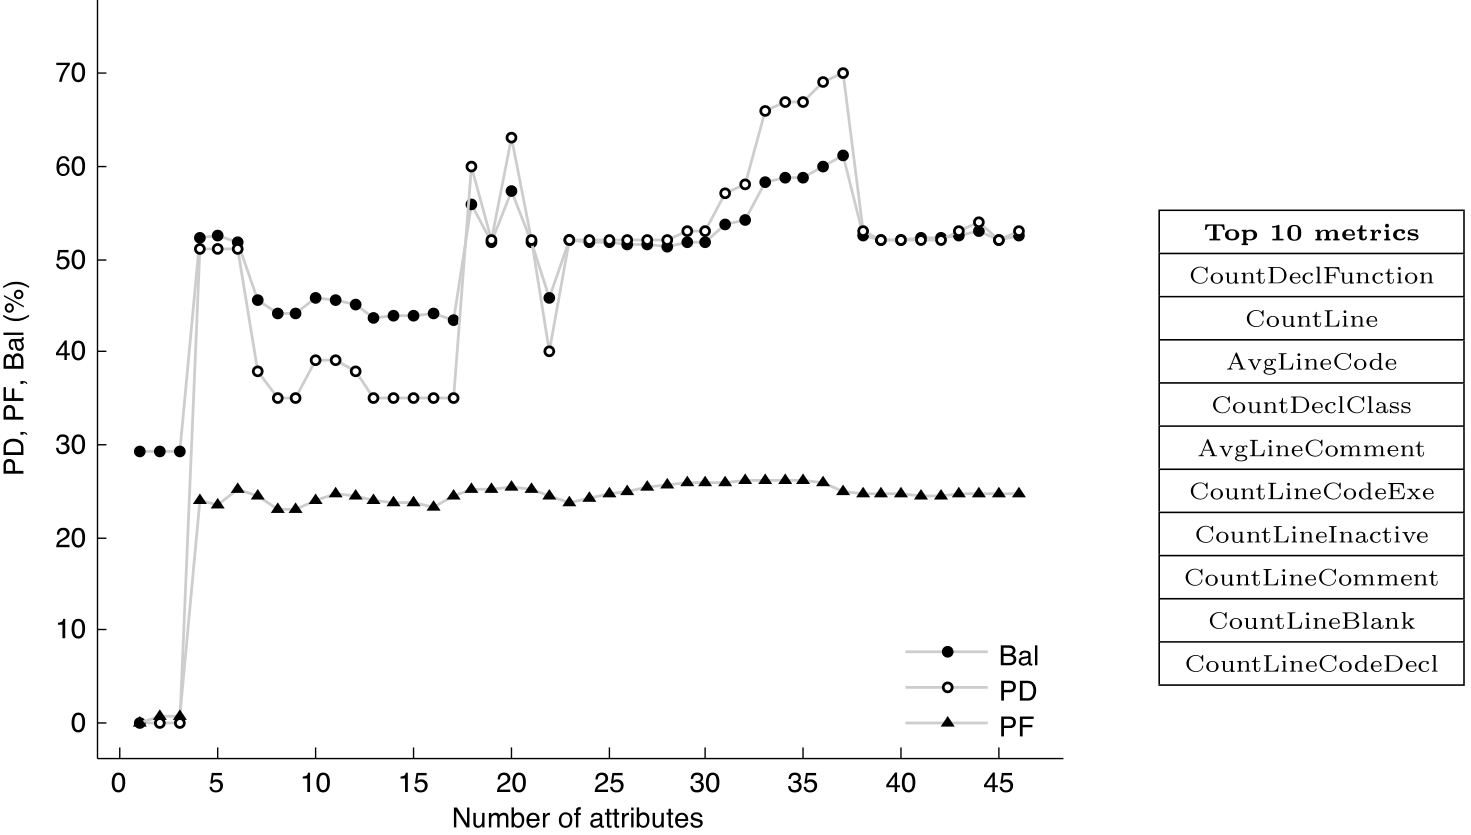
\includegraphics[width=\textwidth]{figures/attributesCardamom.png}
 \end{center}
\end{frame}

\begin{frame}
 \frametitle{Impact of attribute selection}
 \begin{itemize}
  \item Top metrics not the same
  \item Need about 5 top metrics
  \item With all metrics, nearly the same results than with 5
 \end{itemize}
 \vspace{0.5cm}
 \begin{center}
  $\Longrightarrow$ \alert{We keep the full set of metrics.}
 \end{center}
\end{frame}